En esta sección se van a evaluar los entornos de desarrollo más populares: React, Svelte, VueJS, Preact y Angular. Como preámbulo, se muestra en la figura \cref{fig:stjs2019:frontend} la satisfacción de los usuarios con respecto a cada entorno. Esto es relevante porque la satisfacción de los usuarios depende de factores como la eficiencia de código y la curva de aprendizaje. Como queremos que nuestro marco de trabajo esté destinado a aplicaciones pequeñas que tienen potencial para crecer, es importante conocer cuál es la opinión media de los usuarios de 2019. Además queremos que el entorno sea accesible al mayor número de usuarios, por lo que la popularidad es el factor más relevante en este estudio. Prueba: \citet{STJS2019}.

\begin{figure}
	\centering
	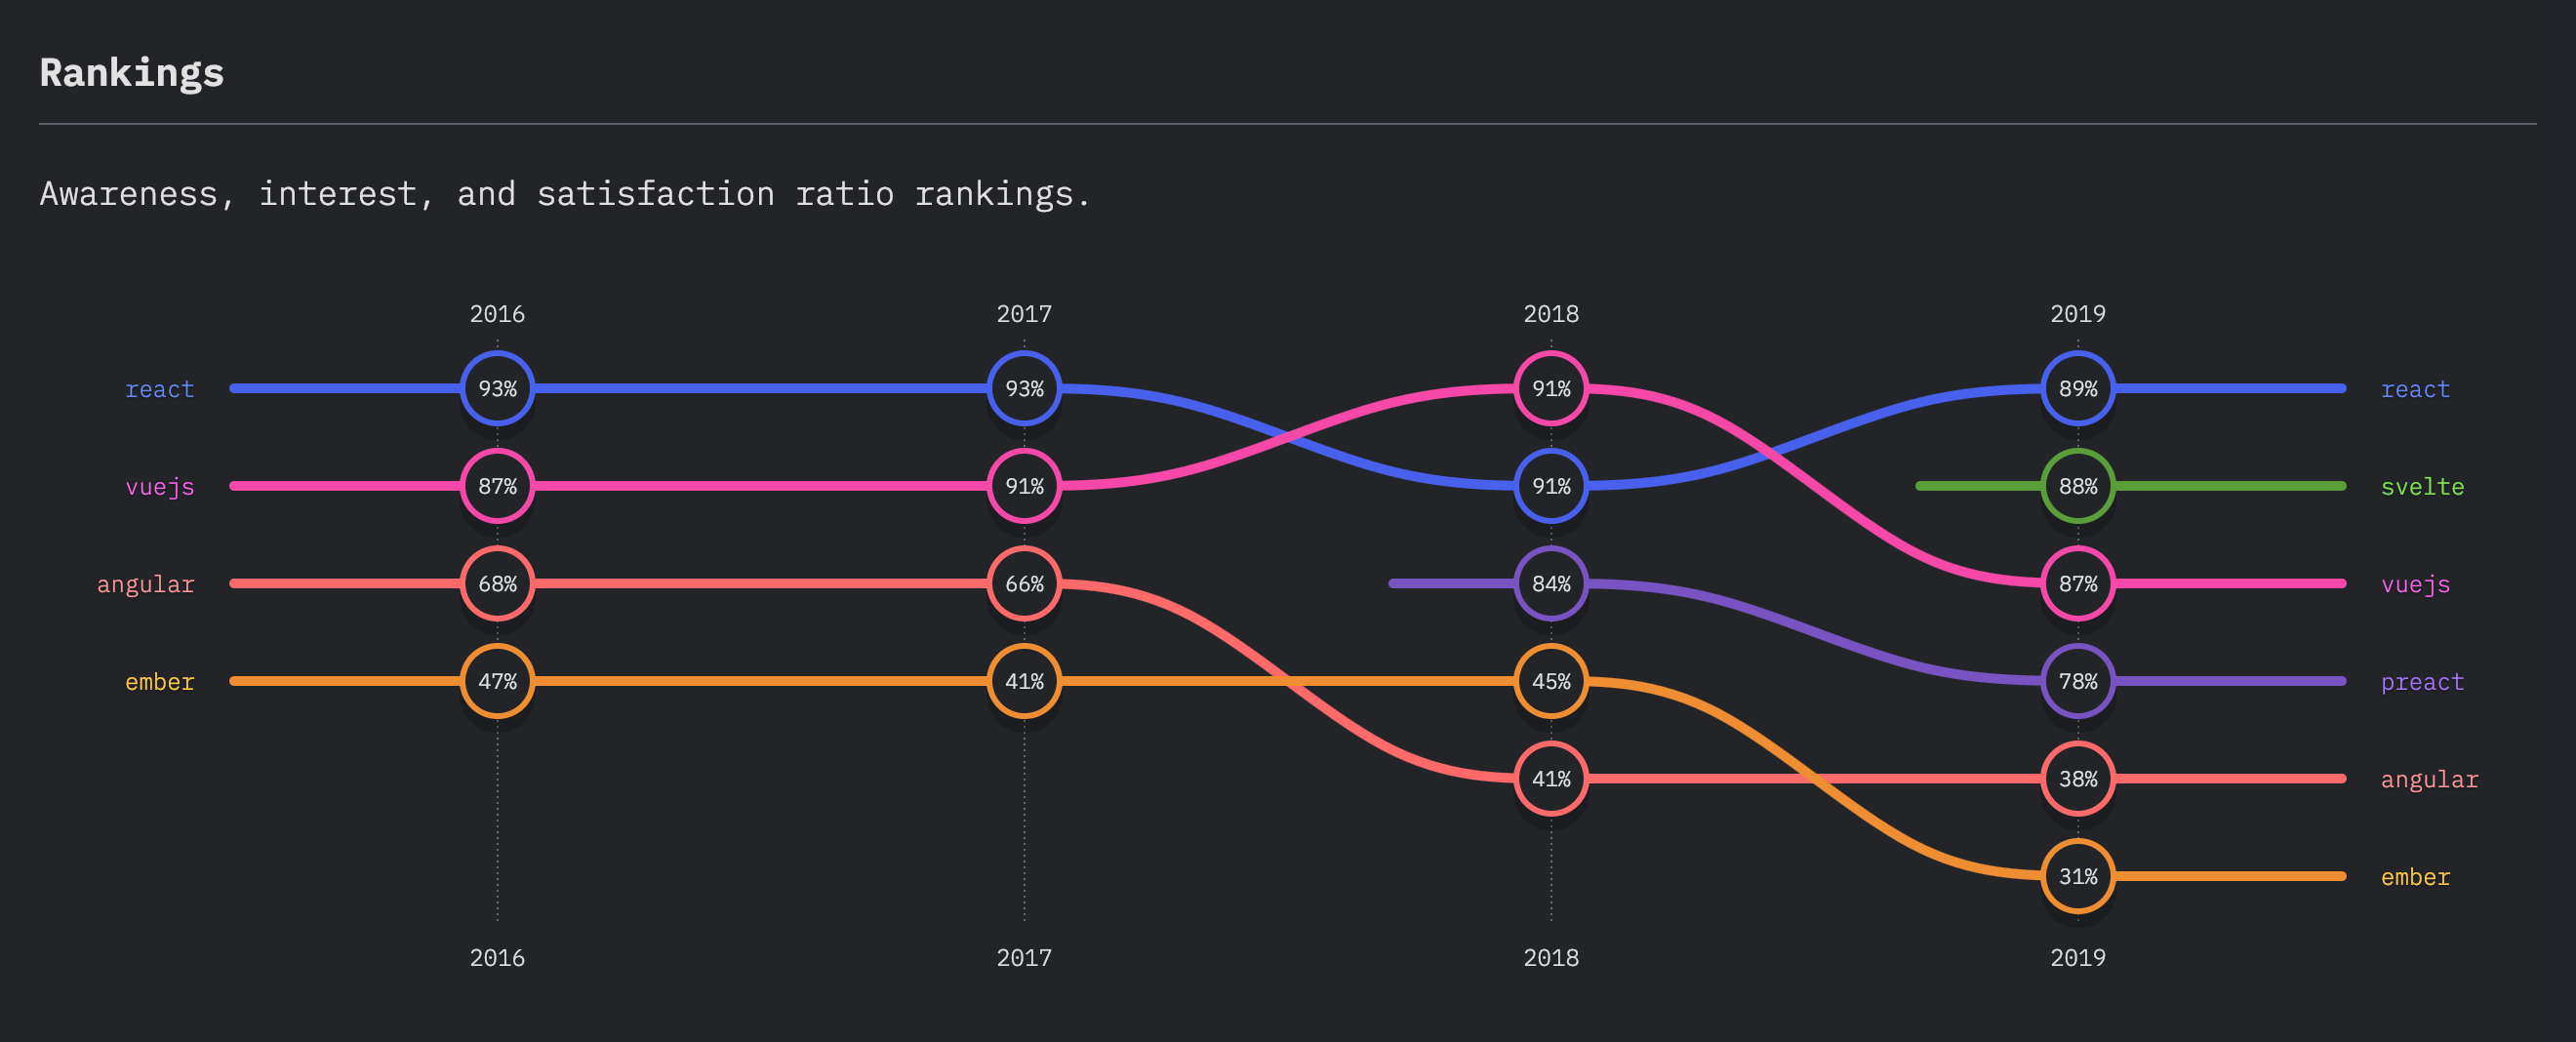
\includegraphics{front_end_frameworks_experience_ranking.png}
	\caption{2019 - Opinión popular de los entornos de trabajo front-end}
	\label{fig:stjs2019:frontend}
\end{figure}